\chapter[Metodologia]{Metodologia}

Inicialmente foi feito um levamento bibliográfico sobre o funcionamento de um forno para tratamento térmico. O grupo foi divido em pequenos times formados por 2, 3 ou 4 integrantes responsáveis por cada área específica do forno. Com isso foi feito um estudo específico de cada módulo para desenvolvimento do trabalho.

A metodologia utilizada será a Top/Down, em que consiste projetar o sistema em uma visão geral fragmentando-o até virar um bloco de menor hierarquia. Espera-se como resultado um passo a passo de cada etapa do projeto, com cada módulo bem detalhado até que se obtenham as especificações do sistema abordado.


\section{Termo de Abertura do Projeto - TAP}

O termo de abertura do projeto foi a primeira atividade feita em conjunto e teve como objetivo melhorar o planejamento do grupo, além de auxiliar na definição do escopo do projeto. No anexo A, encontra-se o modelo preenchido pelo grupo.

\section{Estrutura Analítica de Projeto - EAP}

A estrutura analítica do projeto foi definida baseada nos marcos principais e quais atividades deverão ser entregues. Conforme citado na metodologia Top/Down, as atividades foram divididas em módulos de entrega conforme figura abaixo:

\begin{figure}[!ht]
	\centering
	\label{eap}
	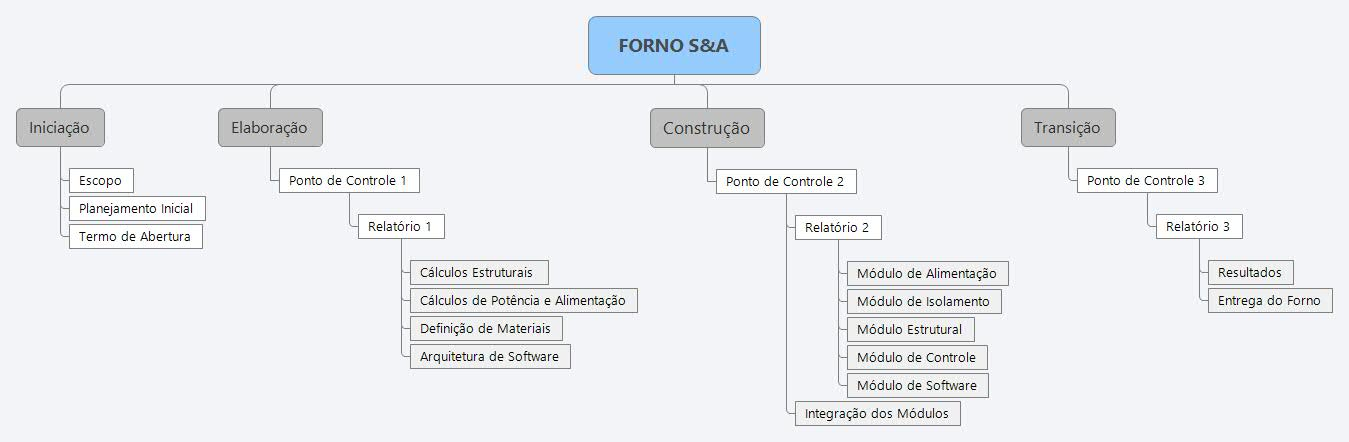
\includegraphics[keepaspectratio=true,scale=0.3]{figuras/eap.jpg}
	\caption{Estrutura Analítica do Projeto.}
\end{figure}

\section{Gerenciamento}

\subsection{Comunicação do Grupo}

A comunicação será feita por meio de ferramentas online como Whatsapp, Facebook, Google Drive, Dropbox e Skype. Além disso, todas às quartas de 16h às 18h e sextas de 14h às 18h de maneira presencial.

\subsection{Divisão dos Recursos Humanos}

A figura a seguir representa o organograma do projeto, no qual foi escolhido um gerente geral e em todos os subgrupos qualquer integrante tem autonomia para exercer o papel de líder.

\begin{figure}[!ht]
	\centering
	\label{rh}
	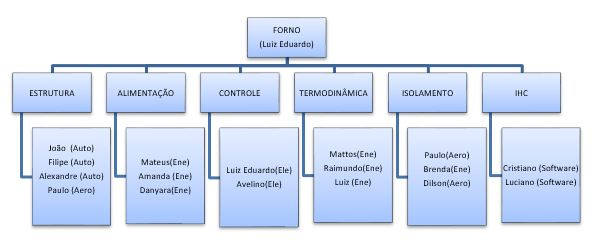
\includegraphics[keepaspectratio=true,scale=1.0]{figuras/rh.JPG}
	\caption{Recursos Humanos do Projeto.}
\end{figure}


\subsection{Custos}

Foi feito um levantamento dos principais materiais que serão utilizados e a seguir temos uma planilha de custo inicial:

\begin{figure}[!ht]
	\centering
	\label{custo}
	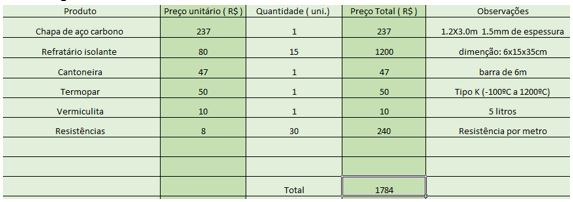
\includegraphics[keepaspectratio=true,scale=0.8]{figuras/custo.JPG}
	\caption{Custo do Projeto.}
\end{figure}

\subsubsection{Orçamento}
Para a aquisição dos produtos, foi feito uma arrecadação de R\$ 80,00 de cada integrante do grupo. Com este valor foi possível obter os principais materiais a serem utilizados, porém para o ponto de controle 3 será feito mais uma arrecadação com o intuito de comprar os materiais que estão faltando.

\begin{figure}[H]
	\centering
	\label{custo}
	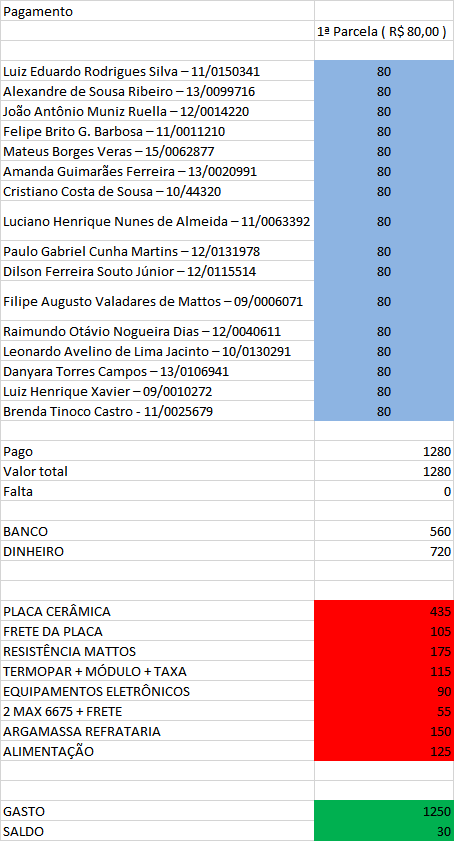
\includegraphics[keepaspectratio=true,scale=0.8]{figuras/orcamento.jpg}
	\caption{Orçamento do Projeto.}
\end{figure}

\subsection{Mapa de Riscos}

O gerenciamento de riscos visa mapear as ameaças e oportunidades que podem influenciar no projeto, positivamente ou negativamente. Com isso, pretende-se propor alternativas que podem reduzir os impactos ocasionados por situações de alto risco, além de otimizar recursos como tempo e custo, caso aconteça alguma oportunidade.

Visando o gerenciamento de riscos, levou-se em consideração as categorias: C – custo; T – tempo e Q – qualidade. Para tal, também foram definidos cinco níveis de probabilidade de ocorrência e de severidade para se verificar em qual categoria o risco se encaixa.

\begin{figure}[!ht]
	\centering
	\label{risco2}
	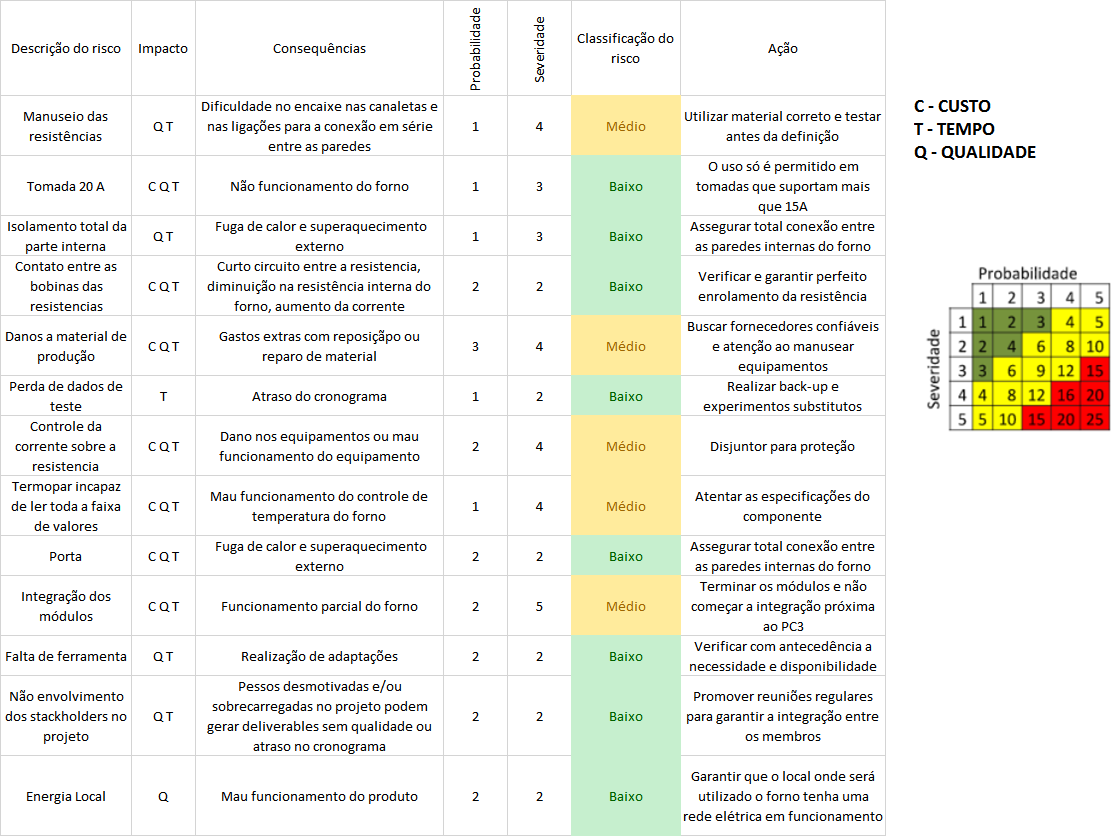
\includegraphics[keepaspectratio=true,scale=0.8]{figuras/riscos.png}
	\caption{Mapa de Riscos.}
\end{figure}

\subsection{Cronograma}

O cronograma do projeto pode ser visualizado na figura a seguir.

\begin{figure}[!ht]
	\centering
	\label{cronograma}
	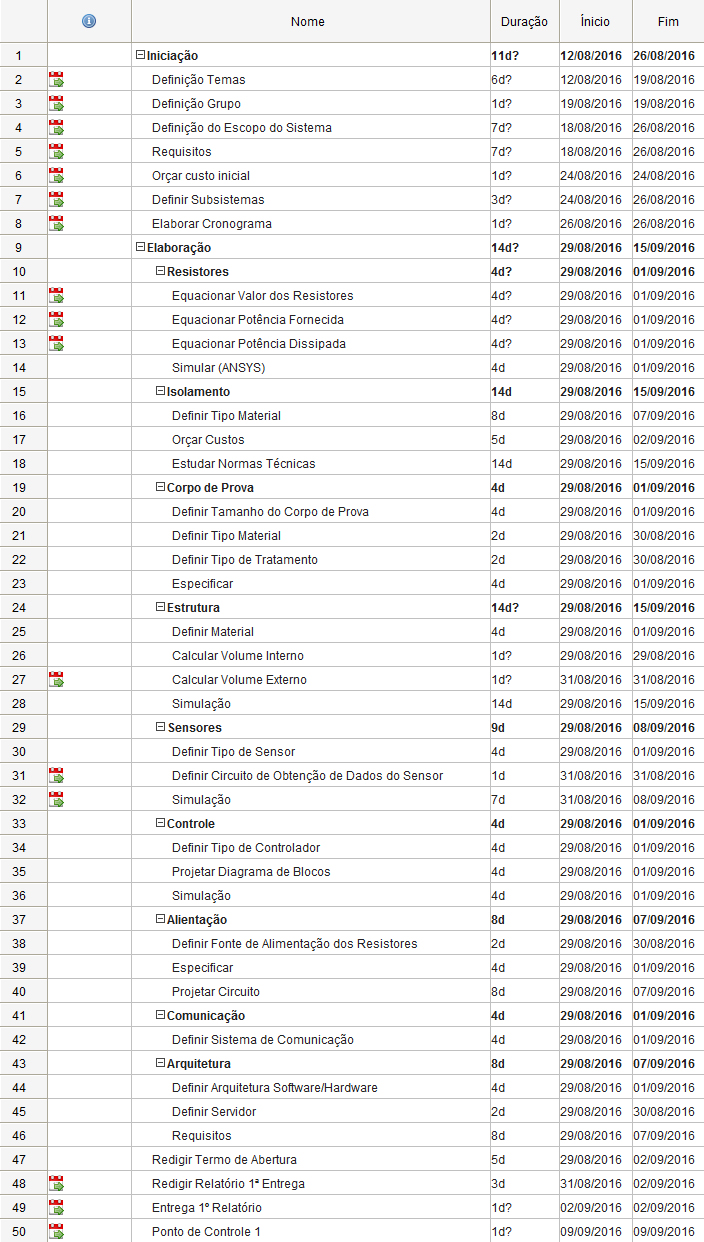
\includegraphics[keepaspectratio=true,scale=0.6]{figuras/cronograma.jpg}
	\caption{Cronograma do Projeto.}
\end{figure}

\begin{figure}[!ht]
	\centering
	\label{cronogramapc2}
	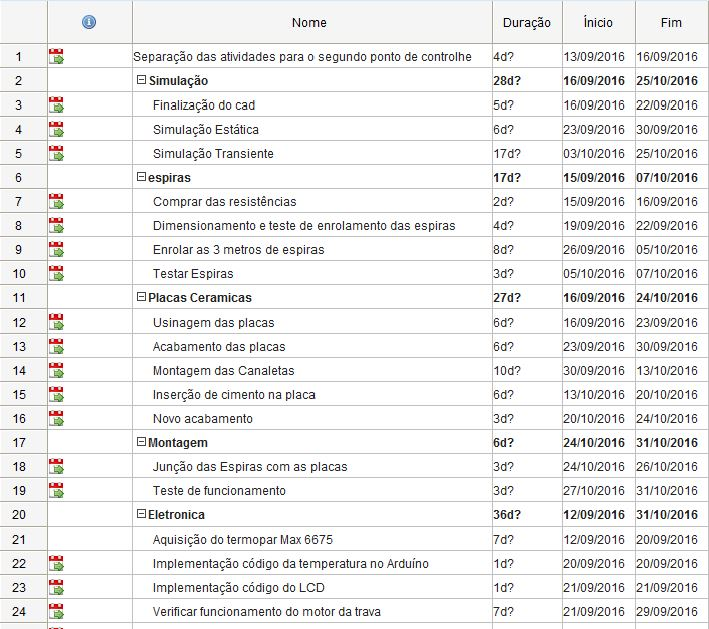
\includegraphics[keepaspectratio=true,scale=0.6]{figuras/cronogramapc2.JPG}
	\caption{Cronograma do Projeto (PC2).}
\end{figure}

\begin{figure}[!ht]
	\centering
	\label{cronogramapc2_cont}
	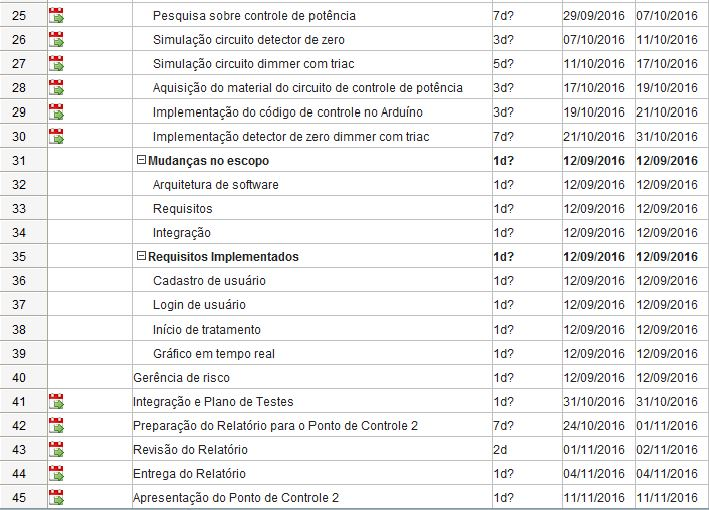
\includegraphics[keepaspectratio=true,scale=0.6]{figuras/cronogramapc2_cont.JPG}
	\caption{Cronograma do Projeto (PC2 - continuação).}
\end{figure}

